\textbf{Note: }\textit{The majority of the work presented in this chapter was published in two independent pieces of work. All work relating to the globular targets was published by \textcite{Simkovic2016-wk}, and a great majority of work relating to the transmembrane targets by \textcite{Thomas2017-sh}. As such, this chapter consists of extracts from both publications with additional information where appropriate. Text duplicated from either publication was written by Felix Simkovic, all other elements were adapted.}

\section{Introduction}
The introduction of residue-residue contacts as distance restraints in \textit{ab initio} protein structure prediction has proven to be a highly successful approach to limiting the conformation search space thereby enabling successful fold prediction of larger and more \textbeta-rich protein structures \cite[e.g.,][]{Marks2011-os,Michel2014-eg,Kosciolek2014-bt,Ovchinnikov2015-tn,Ovchinnikov2016-jj,Michel2017-xh,De_Oliveira2017-sg,Ovchinnikov2017-nd,Wang2017-rx}. In AMPLE, these two domains are the major limitation for a more successful approach \cite{Bibby2012-lm}. This typically results in user success being limited to small globular and primarily \textalpha-helical folds, or time- and resource-demanding attempts most likely going to be unsuccessful for larger targets

With the advent of contact information, is has thus become essential to identify the extend to which this invaluable bit of information is going to help AMPLE users in the future.

\section{Materials \& Methods}
\subsection{Target selection}
In this study, targets from the ORIGINAL and TRANSMEMBRANE datasets were used. This resulted in a final set of 21 globular and 17 transmembrain protein targets. For details in how the targets were selected refer to \cref{sec:methods_dataset_original,sec:methods_dataset_transmembrane}, and for details on each target refer to \cref{table:appendix_dataset_transmembrane,table:appendix_dataset_original}.

\subsection{Contact prediction} \label{sec:ample_proof_conpred}
For all globular targets, one contact map was predicted with the fully automated metapredictor PCONSC2 v1.0 \cite{Skwark2014-qp}. In summary, four \gls{msa}s were generated with JACKHMMER v3.1b2 \cite{Johnson2010-uz} against the \texttt{uniref100} v2015-10 database and HHBLITS v2.0.15 \cite{Remmert2011-kt} against the \texttt{uniprot20} v2013-03 database \cite{Bateman2017-pb} at E-value cutoffs of 10\textsuperscript{-40}, 10\textsuperscript{-10}, 10\textsuperscript{-4} and 1. Each \gls{msa} was analysed with PSICOV v2.13b3 \cite{Jones2012-ks} and PLMDCA v2 \cite{Ekeberg2014-kf} to produce 16 individual contact predictions. All 16 predictions and per-target PSIPRED v3 \cite{Jones1999-ed} secondary structure prediction, NETSURFP v1.0 \cite{Petersen2009-wy} solvent accessibility information and HHBLITS v2.0.15 \cite{Remmert2011-kt} sequence profile were provided to the PCONSC2 deep learning algorithm \cite{Skwark2014-qp} to identify protein-like contact patterns. The latter produced a final contact map for each target sequence.

An additional contact map for \textbeta-structure containing targets was predicted using CCMPRED v0.3 \cite{Seemayer2014-zp} and reduced to \textbeta-sheet contact pairs using the CCMPRED-specific filtering protocol BBCONTACTS v1.0 \cite{Andreani2015-qn}. Each \gls{msa} for CCMPRED contact prediction was obtained using HHBLITS v2.0.15 \cite{Remmert2011-kt}. This entailed two sequence search iterations with an E-value cutoff of 10\textsuperscript{-3} against the \texttt{uniprot20} v2013-03 database \cite{Bateman2017-pb} and filtering to 90\% sequence identity using HHFILTER v2.0.15 \cite{Remmert2011-kt} to reduce sequence redundancy in the \gls{msa}. Besides the contact matrix as input, BBCONTACTS requires a secondary structure prediction and an estimate of the \gls{msa} diversity. The secondary structure prediction was taken from the PCONSC2 step whilst the diversity factor was calculated using \cref{eq:methods_alndiversity}.

For each transmembrane protein target, a \gls{msa} was generated using HHBLITS v2.0.16 \cite{Remmert2011-kt} against \texttt{uniprot20} v2016-02 database \cite{Bateman2017-pb}. Contact predictions for each transmembrane target were obtained using the metapredictor METAPSICOV v1.04 \cite{Jones2015-vq}, which in turn used the contact prediction algorithms CCMPRED v0.3.2 \cite{Seemayer2014-zp}, FREECONTACT v1.0.21 \cite{Kajan2014-bx} and PSICOV v2.1b3 \cite{Jones2012-ks}. Additionally, a set of contacts was also generated using the MEMBRAIN server v2015-03-15 \cite{Yang2013-bf}.

\subsection{Contact-to-restraint conversion} \label{sec:bbcontacts_addition}
For all targets, the predicted contact maps were converted to ROSETTA restraints to guide \textit{ab initio} structure prediction. The FADE energy function was used to introduce a restraint in ROSETTA's folding protocol. The implementation described by \textcite{Michel2014-eg} was used, which defined a contact to be formed during folding if the participating C\textbeta\ atoms (C\textalpha\ in case of glycine) were within 9\AA\ of one another. The top-$L$ ($L$ corresponds to the number of residues in the target sequence) contact pairs were converted to ROSETTA restraints, and if satisfied a ``squared-well'' bonus of -15.00 added to the energy function.

Additionally to above, all \textbeta-containing targets were subjected to a further conversion step in a separate condition. The approach of adding BBCONTACTS restraints to a previous prediction is outlined in \cref{sec:methods_bbcontacts_addition}.

\subsection{\textit{Ab initio} structure prediction}
Fragments for all targets were selected using the \texttt{make\_fragments.pl} script shipped with ROSETTA. To ensure no homologous fragments were included in the fragment libraries, the \texttt{-nohoms} flag was set. Each target's secondary structure prediction was provided to the fragment picker using the \texttt{-psipredfile} argument. The fragment libraries, contact restraints and secondary structure prediction were subjected to the ROSETTA \texttt{AbinitioRelax} protocol \cite{Rohl2004-dj} to predict 1,000 decoys per target. ROSETTA options were chosen according to the default protocol in AMPLE v1.0 \cite{Bibby2012-lm}. ROSETTA v2015.05.57576 was used for globular targets and v2015.22.57859 for transmembrane ones for all ROSETTA-related protocols.
%
\subsection{Molecular Replacement in AMPLE}
All generated decoys were subjected to AMPLE v1.0 \cite{Bibby2012-lm} for ensemble search model generation. 

All transmembrane protein targets were processing using AMPLE's default parameters. \Gls{mr} trials were performed with software versions shipped in CCP4 v6.5.13 \cite{Winn2011-xe}, with the exception of SHELXE v2014/14 \cite{Thorn2013-le} and ARP/wARP v7.5 \cite{Cohen2007-wg}.

All globular protein targets were subjected to AMPLE with two deviations from the default parameters. The \texttt{-use\_scwrl} was set to subject all decoys to side-chain remodelling using SCWRL4 \cite{Krivov2009-ex}. Furthermore, the number of clusters to trial was set increased from one to three via the \texttt{-num\_clusters}parameter. All \gls{mr} trials were performed with the version of software shipped with CCP4 v6.5.15 \cite{Winn2011-xe}.

All \gls{mr} solutions were assessed for success using the criteria described in \cref{sec:methods_mr_success}.

\section{Results}
In this study, the application of residue-residue contact predictions to \textit{ab initio} protein structure prediction and subsequently \gls{mr} was investigated. This proof-of-concept work is based on two datasets covering a range of globular and transmembrane protein targets. At the time of conducting this study, state-of-the-art contact prediction algorithms were applied to obtain the best possible contact predictions to identify the extend of pushing the boundaries previously incurred in AMPLE studies \cite{Bibby2012-lm}.

\subsection{Residue-residue contact prediction}
Accurate coevolution-based residue-residue contact prediction is highly dependent on the availability of many divergent homologous sequences. As such, it is important to validate that the selected targets in this study satisfy such requirement.

The depth of \gls{msa}s obtained for each target sequence suggests that sufficient numbers of divergent homologous sequences are available. Across all globular targets, the minimum alignment depth is obtained for Galectin-3 domain (\gls{pdb} ID: 1kjl) with 679 effective sequences and the maximum for G-protein Arf6-GDP (\gls{pdb} ID: 1e0s) with 1,897 effective sequences (\cref{fig:ample_proof_globpreccomp}). The median alignment depth for all globular targets is over 1,000, which is beyond the often suggested threshold of 200 sequences \cite{Simkovic2017-xs}. The \gls{msa}s for all transmembrane protein targets also surpass this threshold comfortably. The median alignment depth is much higher than for globular targets with 1,878 sequences (\cref{fig:ample_proof_tmpreccomp}). The minimum, which was obtained for Sensory rhodopsin II (\gls{pdb} ID: 1gu8), is 692 sequences and the maximum for the sequence of Rhomboid protease GLPG (\gls{pdb} ID: 2xov) is 6,583.

\begin{figure}[H]
    \centering
    \begin{subfigure}[b]{\textwidth}
        \centering
        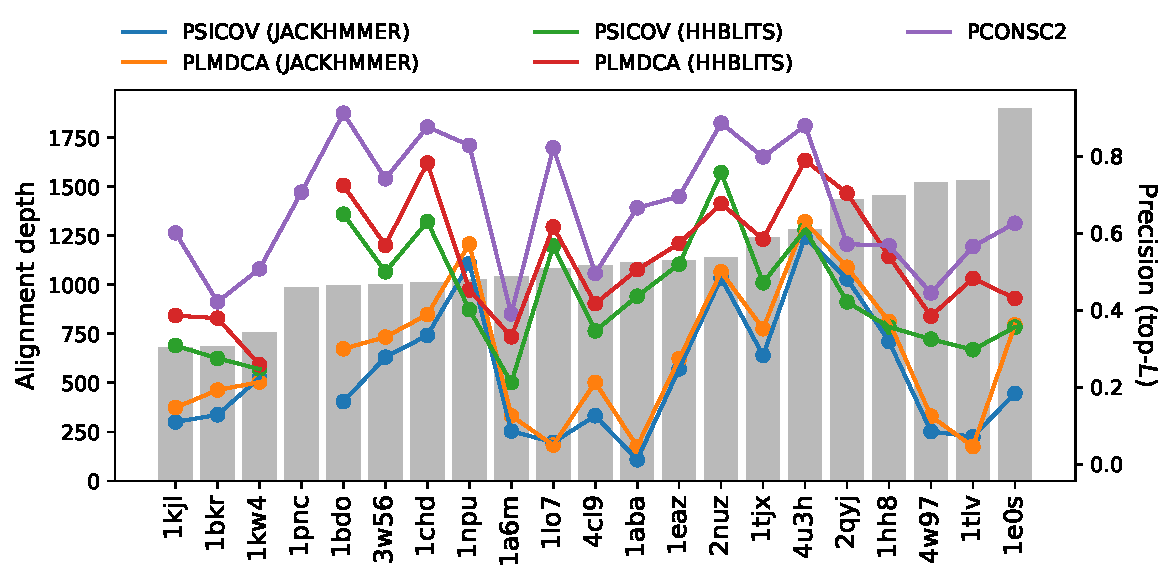
\includegraphics[width=\textwidth]{ample_proof_globpreccomp.pdf}
        \caption{}
        \label{fig:ample_proof_globpreccomp}
    \end{subfigure}
    
    \begin{subfigure}[b]{\textwidth}
        \centering
        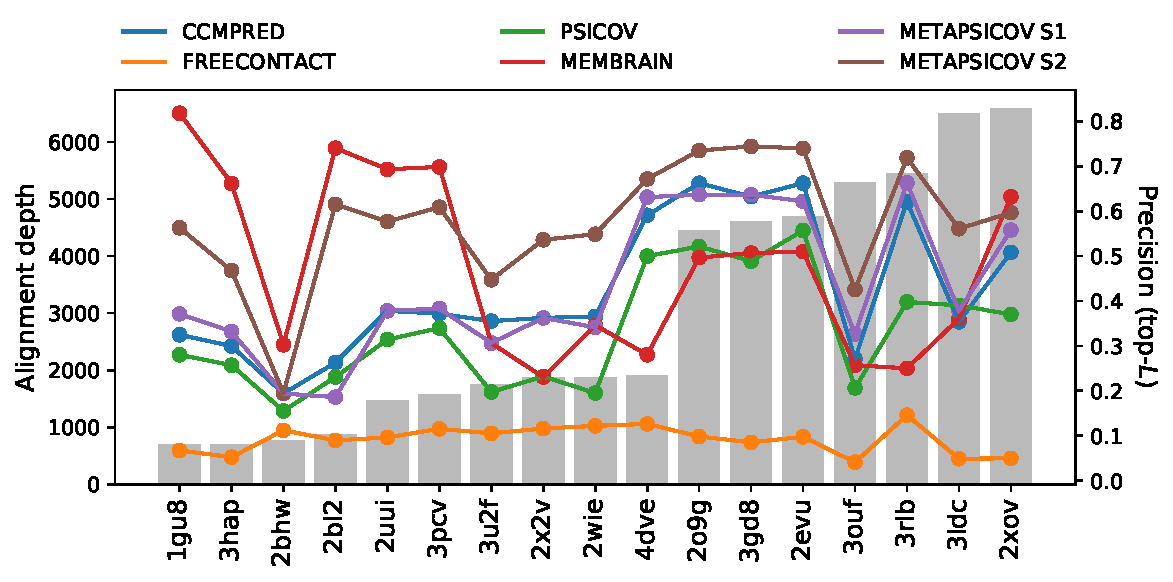
\includegraphics[width=\textwidth]{ample_proof_tmpreccomp.pdf}
        \caption{}
        \label{fig:ample_proof_tmpreccomp}
    \end{subfigure}
    
    \caption[Alignment depth and contact precision analysis of globular and transmembrane protein targets]{Alignment depth and contact precision analysis of (a) globular and (b) transmembrane protein targets. Contact predictions were obtained with several contact prediction algorithms. Precision scores were calculated for the top-$L$ contact pairs. JACKHMMER and HHBLITS alignments for PSICOV and PLMDCA contact predictions in (a) were obtained with E-value $1e^{-4}$.} 
    \label{fig:ample_proof_preccomp}
\end{figure}

In coevolution-based contact prediction, the precision depends on alignment depth. Despite sufficient number of effective sequences across all targets, findings in this study suggest that some (meta-)predictors cannot fully utelise greater alignment depths to correct contact pairs (\cref{fig:ample_proof_preccomp}). 

PCONSC2 --- a metapredictor using numerous starting alignments and two contact predictors --- outperforms its individual parts for almost all globular targets (\cref{fig:ample_proof_globpreccomp}). Despite only a fraction of all generated contact predictions illustrated in \cref{fig:ample_proof_globpreccomp}, the pattern translates across all 16 predictions per target. Such results suggest that precision greatly depends on the tool used to identify and select homologous sequences for the \gls{msa}. A closer inspection of mean precision scores resulting from HHBLITS- and JACKHMMER-based alignments shows higher precision scores for top-$L$ contact pairs based on the former alignments (\cref{table:ample_proof_pconsc2}). Nevertheless, the Machine Learning approach in PCONSC2 to combine more and less precise individual predictions results in superior precision in the output (\cref{table:ample_proof_pconsc2}). No correlation could be established between alignment depth and precision for either individual predictors or the metapredictor PCONSC2 (\cref{fig:ample_proof_globpreccomp}). 

\begin{table}[H]
    \centering
    \caption[Summary of raw conact prediction precision values in PCONSC2]{Summary of mean PCONSC2 raw contact prediction precision based on JACKHMMER and HHBLITS alignments and PSICOV, PLMDCA and PCONSC2 coevolution-based contact prediction.}
    \label{table:ample_proof_pconsc2}
    \begin{tabularx}{\textwidth}{b b s s s s}
        \hline
        \multicolumn{2}{c}{\textbf{Contact prediction}} & \multicolumn{4}{c}{\textbf{Alignment E-value cutoff}} \\
        \cline{3-6} & & $1e^{0}$ & $1e^{-4}$ & $1e^{-10}$ & $1e^{-40}$ \\ 

        \hline
        \multirow{2}{1em}{PSICOV} & JACKHMMER  & 0.240 & 0.239 & 0.213 & 0.167 \\
                                  & HHBLITS    & 0.439 & 0.435 & 0.354 & 0.209 \\
        \hline
        \multirow{2}{1em}{PLMDCA} & JACKHMMER  & 0.293 & 0.288 & 0.252 & 0.140 \\ 
                                  & HHBLITS    & 0.545 & 0.530 & 0.447 & 0.224 \\
        \hline
        \hline
        PCONSC2                   &            & \multicolumn{4}{c}{0.667}     \\
        \hline
    \end{tabularx}
\end{table}

Contacts for transmembrane protein targets in this study were predicted with the metapredictor METAPSICOV and the transmembrane-specific predictor MEMBRAIN. METAPSICOV STAGE 1 and STAGE 2 predictions outperform MEMBRAIN in nine and ten cases, respectively, whilst MEMBRAIN outperforms METAPSICOV for the rest (\cref{fig:ample_proof_tmpreccomp}). The METAPSICOV algorithm utelises the raw predictions by CCMPRED, FREECONTACT and PSICOV to generate its STAGE 1 and STAGE 2 predictions. METAPSICOV STAGE 1 predictions are near identical to CCMPRED, whereby 15 of 17 targets show an absolute $\Delta_{TMscore}$ of less than 0.05 (\cref{fig:ample_proof_tmpreccomp}). This similarity does not propagate to METAPSICOV STAGE 2 predictions with only a single target showing such similar \gls{tmscore} values (\cref{fig:ample_proof_tmpreccomp}). Amongst the three raw predictors used by METAPSICOV, FREECONTACT performs by far the worst with a mean \gls{tmscore} of 0.09 across all transmembrane targets. PSICOV shows similar trend to CCMPRED when assessed by target, which results in a mean absolute $\Delta_{TMscore}$ of 0.10.

The addition of BBCONTACTS contact pairs to improve structure prediction accuracy for \textbeta-structure containing targets is a novel aspect introduced in this study. The initial step of the addition of BBCONTACTS contact pairs included the filtering of one- and two-pair strand contacts from the original BBCONTACTS list, since those contained high numbers of false positives (Jessica Andreani, personal communication). The findings in this study confirm this for all \textbeta-structure containing targets. Precision values improved for all targets with changes ranging from 0.01 to 0.14 whilst retaining on average 80\% of all contacts. Filtered BBCONTACTS predictions were combined with other contact maps, i.e. PCONSC2, to either upweight or add contact pairs. Findings in this study highlight that upweighted contact pairs are more precise than ones to be added. The minimum precision score for a set of upweighted contacts is 0.72 for 29 contact pairs and the maximum of 1.00 for up to 27 contact pairs. In comparison, novel BBCONTACTS contact pairs not present in the base contact map range in precision scores from 0.22 (nine contacts) to 0.76 (21 contacts). 

\begin{figure}[H]
    \centering
    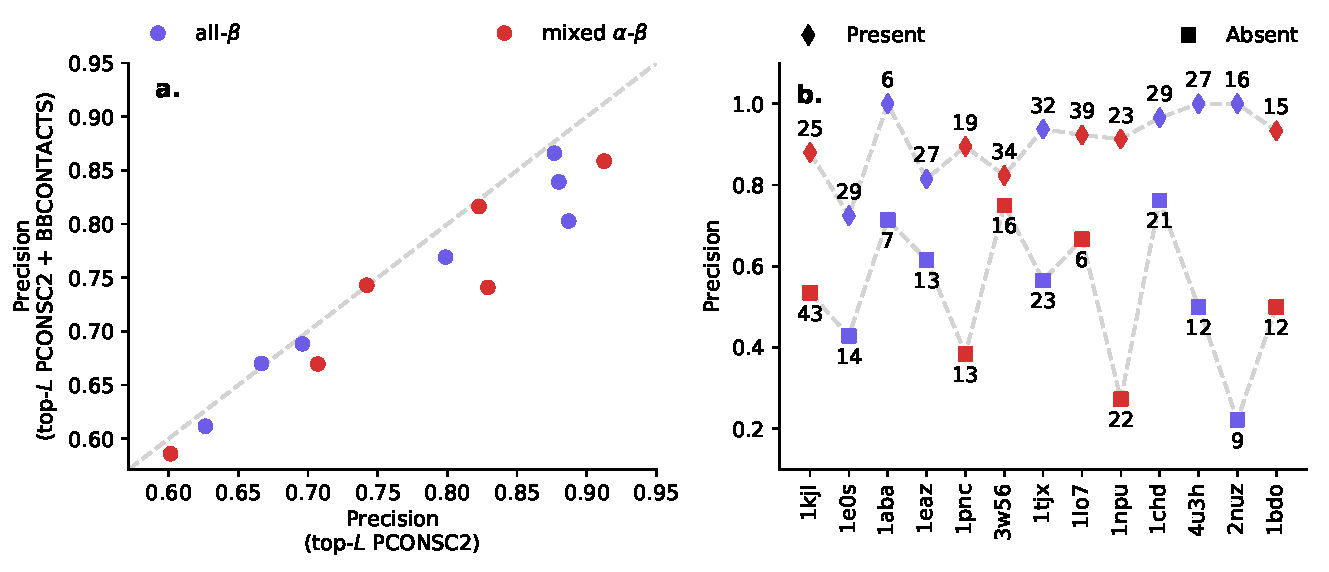
\includegraphics[width=\textwidth]{ample_proof_bbaddon.pdf}
    \caption[Evaluation of BBCONTACTS contact pairs]{Evaluation of BBCONTACTS contact pairs. (a) Precision evaluation of PCONSC2 contact map with and without BBCONTACTS. (b) Precision evaluation of BBCONTACTS contact pairs split by status of presence or absence in the base PCONSC2 contact list. Numbers besides each marker indicate the number of contacts. The order scatter points is identical between both subplots and based on the PCONSC2 precision values (x-axis) in (a).}
    \label{fig:ample_proof_bbaddon}
\end{figure}

Despite the high precision of BBCONTACTS contact pairs, the merge of such pairs with top-$L$ PCONSC2 contact pairs results in an expected loss in precision for the resulting contact set (\cref{fig:ample_proof_bbaddon}). True positive contacts, which dominate the BBCONTACTS contact set, are usually also predicted by PCONSC2, and thus upweighted (\cref{fig:ample_proof_bbaddon}). Since upweighting does not affect the precision, the value remains unaffected after this procedure. However, contact pairs unique to BBCONTACTS contact more false positives. Once added to the base PCONSC2 contact list, these contacts therefore reduce the precision value (\cref{fig:ample_proof_bbaddon}). Either subset of BBCONTACTS contacts does not show any correlation between the number it contains and its precision. The fold of the target does not show any clear distinction between better and worse sets of contacts either (\cref{fig:ample_proof_bbaddon}).

\subsection{Protein structure prediction}

Predicted contact information is particularly useful to limit the conformation search space in \textit{ab initio} protein structure prediction. Since such predictions are the basis for AMPLE studies presented in this thesis, it is important to analyse the improvement in decoy quality.

Globular protein targets benefit greatly from the addition of PCONSC2 residue contacts. All but one target see median \gls{tmscore} improvements of at least 0.05 when comparing contact-guided PCONSC2 decoys with simple ROSETTA decoys (\cref{fig:ample_proof_comproscon}). The greatest improvement over 1,000 decoys was achieved for Oxy-myoglobin (\gls{pdb} ID: 1a6m) with an improvement in median \gls{tmscore} of 0.42.  The decoys for Ankyrin (\gls{pdb} ID: 2qyj) show a minor decrease in median \gls{tmscore} of 0.04; however, the median \gls{tmscore} for ROSETTA decoys is 0.78, and thus a minor decrease may be negligible. 

\begin{figure}[H]
    \centering
    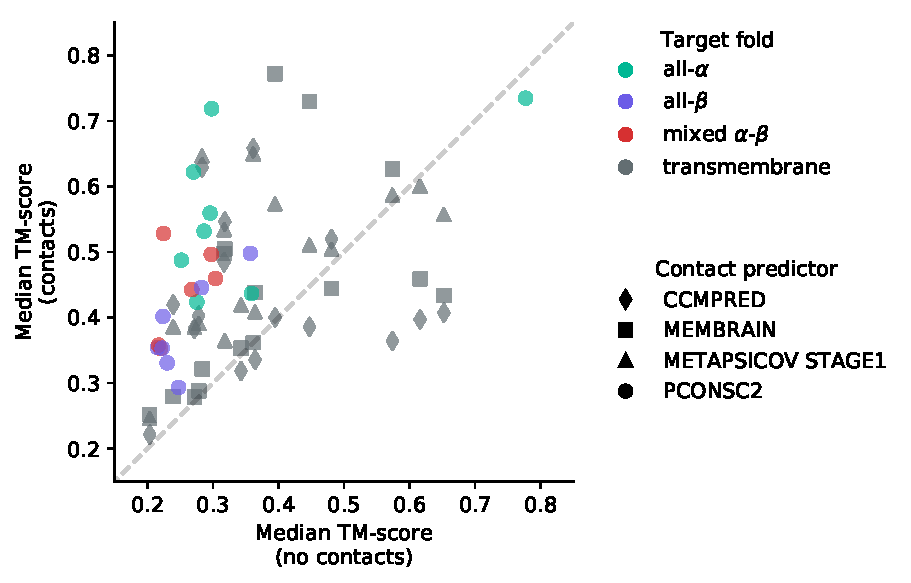
\includegraphics[width=\textwidth]{ample_proof_comproscon.pdf}
    \caption[Effect of contact distance restraints on \textit{ab initio} decoy quality]{Effect of contact distance restraints on \textit{ab initio} decoy quality by comparison of unrestrained (\textit{no contacts}) and contact-restrained (\textit{contacts}) median TM-scores for 1,000 decoys per target. Colours indicate the target fold and symbols the contact prediction algorithm.}
    \label{fig:ample_proof_comproscon}
\end{figure}

Previously, \textit{ab initio} protein structure prediction for globular targets was greatly limited by target fold and chain length. The addition of residue-residue contacts enhances decoy quality primarily for \textalpha-helical and mixed \textalpha-\textbeta\ protein targets (\cref{fig:ample_proof_globtmcomp}). Whilst only one all-\textalpha\ target has more than 50\% native-like decoys in its ROSETTA decoy set, five targets surpass this threshold when PCONSC2 contact data is used to restrain the folding procedure. Similarly, the median \gls{tmscore} of no mixed \textalpha-\textbeta\ target decoy set surpasses the \gls{tmscore} threshold of 0.5 with ROSETTA decoys compared to one for PCONSC2 decoys with three further ones greater than 0.4. All-\textbeta\ targets also benefit from the addition of contact restraints, although decoy sets do not surpass the native-like threshold by median \gls{tmscore} (\cref{fig:ample_proof_globtmcomp}). Larger targets do not benefit any more than smaller targets from the addition of residue contacts to the structure prediction protocol. The only real exception to this are the decoys for the CheB methylesterase domain (\gls{pdb} ID: 1chd), for which the majority of ROSETTA decoys are almost random-like whilst PCONSC2 decoys are native-like (\cref{fig:ample_proof_globtmcomp}).

\begin{figure}[H]
    \centering
    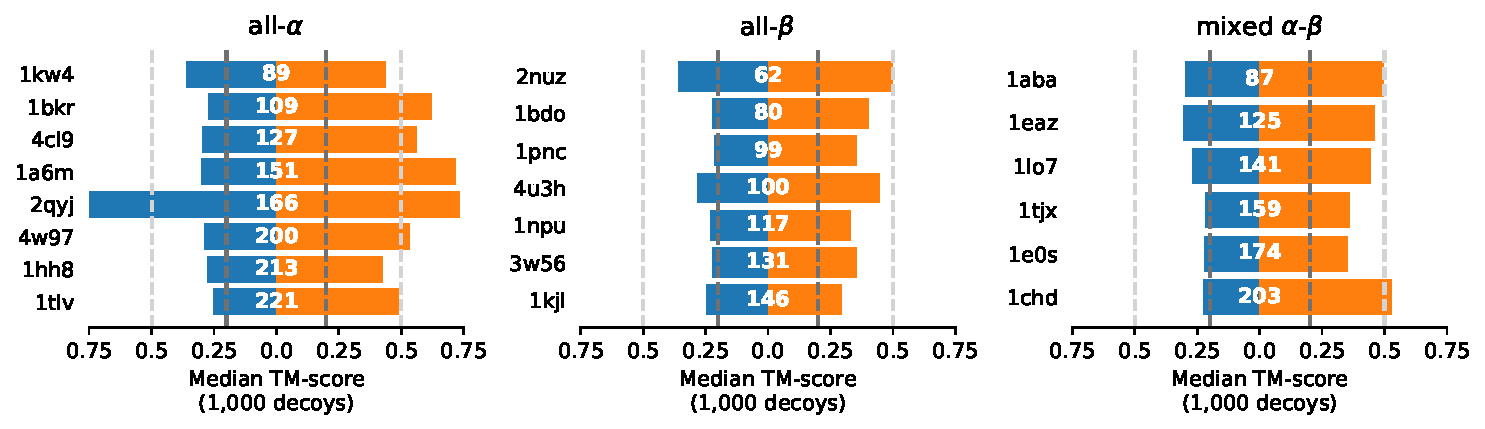
\includegraphics[width=\textwidth]{ample_proof_globtmcomp.pdf}
    \caption[TM-score comparison for globular targets separated by fold]{\gls{tmscore} comparison for globular targets separated by fold and ordered by target chain length. Median \gls{tmscore}s for 1,000 decoys generated with simple ROSETTA (orange) or contact-guided ROSETTA (blue) runs. White numbers in each row correspond to the target chain length. Bars surpassing the dark gray line indicate that the majority of structures are better than random, whilst the light gray line indicates that the majority of structures are native-like \cite{Xu2010-kr}.}
    \label{fig:ample_proof_globtmcomp}
\end{figure}

The enhancement of \textbeta-structure specific contact pairs is an important part of this study. Previously, the precision of the added BBCONTACTS contact pairs has been demonstrated. The next essential step is to explore how the BBCONTACTS supplement enhances or degrades decoy quality after ROSETTA \textit{ab initio} protein structure prediction. Given 13 \textbeta-structure containing targets, eight targets achieve better overall decoy quality with added BBCONTACTS (\cref{fig:ample_proof_comprosconbb}). The smallest improvement is observed for target 1e0s with 0.01 \gls{tmscore} units, whilst the largest for target 1eaz with 0.05 units. The remaining five targets --- \gls{pdb} IDs 1chd, 1bdo, 1npu, 4u3h and 1tjx --- saw decreases in median \gls{tmscore} up to 0.03 when BBCONTACTS contact pairs were added as restraints (\cref{fig:ample_proof_comprosconbb}). No clear difference between fold classes, i.e. mixed \textalpha-\textbeta\ or all-\textbeta\ targets, could be observed, although mixed \textalpha-\textbeta\ targets do show slightly greater extremes (\cref{fig:ample_proof_comprosconbb}).

\begin{figure}[H]
    \centering
    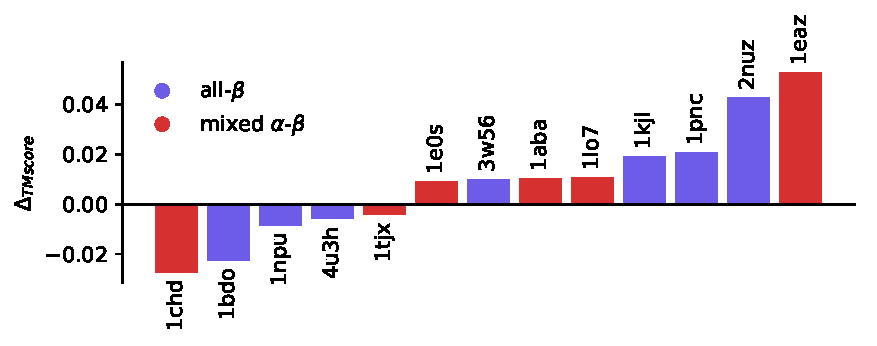
\includegraphics[width=\textwidth]{ample_proof_comprosconbb.pdf}
    \caption[TM-score comparison for \textbeta-richt targets]{\gls{tmscore} comparison for \textbeta-structure containing globular targets separated by fold and ordered by the difference in median \gls{tmscore} between PCONSC2 and PCONSC2+BBCONTACTS decoys. Positive values indicate a better median \gls{tmscore} in favour of PCONSC2+BBCONTACTS decoys, whilst negative values those for PCONSC2. \Gls{pdb} IDs are provided alongside each bar.}
    \label{fig:ample_proof_comprosconbb}
\end{figure}

\textcolor{red}{Something on local features restrained by BBCONTACTS \ldots}

Transmembrane protein targets were modelled using residue-residue contact predictions derived with CCMPRED, MEMBRAIN and METAPSICOV STAGE1. A ROSETTA benchmark was also run to compare contact-guided decoys to the current norm. Findings in this study highlight the much improved decoy quality for almost all targets when contact information is used to reduce the conformational sampling space (\cref{fig:ample_proof_comproscon}). Across all methods, only two targets suffered from the addition of contact restraints during \textit{ab initio} protein structure prediction, namely the domains of ATP synthase C chain (\gls{pdb} ID: 2wie) and ATP synthase subunit C (\gls{pdb} ID: 3u2f). In both cases, ROSETTA generates decoys with median \gls{tmscore} of greater than 0.6 when no contact restraints are used. This contrasts strongly with contact-guided decoy sets, for which only METAPSICOV STAGE1 guide the modelling sufficiently to obtain overall native-like decoys, i.e. median TM-score of greater than 0.5. 

\begin{figure}[H]
    \centering
    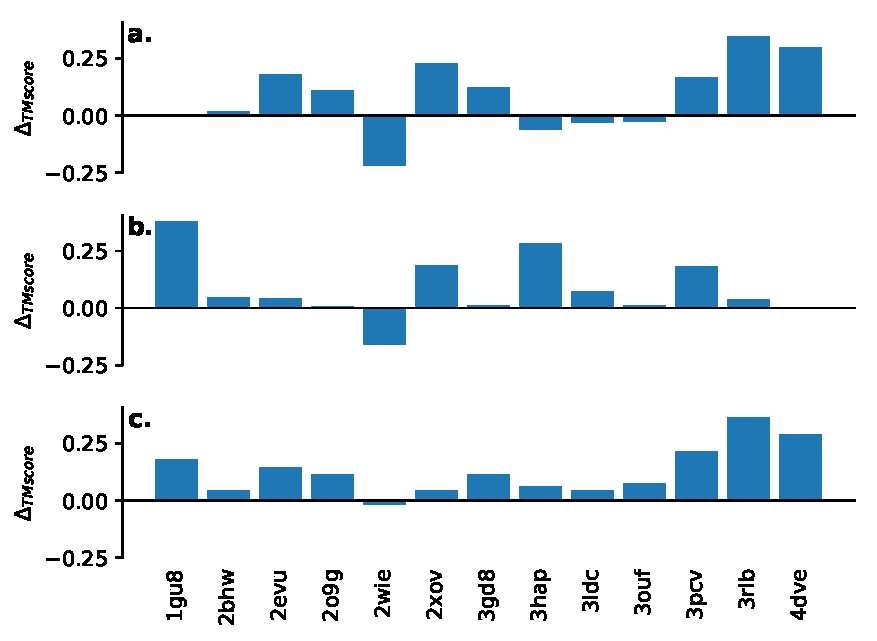
\includegraphics[width=\textwidth]{ample_proof_tmtmcomp.pdf}
    \caption[TM-score difference between contact-guided and simple ROSETTA decoys]{TM-score difference between contact-guided and simple ROSETTA decoys for transmembrane protein targets. Positive $\Delta_{TMscore}$ values indicate more accurate contact-guided decoys, whilst negative values better decoys without the addition of contacts. $\Delta_{TMscore}$ values were computed by median \gls{tmscore}. Contact restraints were obtained with (a.) CCMPRED, (b.) MEMBRAIN, and (c.) METAPSICOV STAGE1.}
    \label{fig:ample_proof_tmtmcomp}
\end{figure}

A split for decoy quality comparison between no-contact and contact-guided decoy sets by contact prediction algorithm shows that CCMPRED contacts are not sufficiently precise to always improve decoy quality. Six out of 16 targets are predicted more accurately without CCMPRED contact information (\cref{fig:ample_proof_tmtmcomp}). In comparison, MEMBRAIN and METAPSICOV STAGE1 contact predictions result in enhanced decoy quality to the extend that only three and two decoy sets are worse than their no-contact counterparts (\cref{fig:ample_proof_tmtmcomp}). Most notably, either of the three contact predictions per target performs better for certain targets. The most extreme example may be the decoy sets for Bacteriorhodopsin (\gls{pdb} ID: 3hap) for which CCMPRED contacts result in decoy quality degradation of 0.06, METAPSICOV STAGE1 in a slight improvement of 0.06 and MEMBRAIN in an improvement of 0.28 \gls{tmscore} units. This translates into absolute decoy counts with native-like fold --- i.e., \gls{tmscore} $\geq 0.5$ --- of the follwing: 274 for decoys without contact guidance, 289 for CCMPRED contact guidance, 538 for METAPSICOV STAGE1 contact guidance, and 996 for MEMBRAIN contact guidance. Similar examples exist (e.g., \gls{pdb} IDs 1gu8, 3rlb or 4dve in \cref{fig:ample_proof_tmtmcomp}) and highlight that no single method yields the best decoys in all circumstances.

\subsection{Molecular Replacement}

Hello World \ldots
